\documentclass[a4paper, 12pt, final, garamond]{book}
\usepackage{cours-preambule}

\raggedbottom

\makeatletter
\renewcommand{\@chapapp}{M\'ecanique -- chapitre}
\makeatother

% \toggletrue{student}
% \HideSolutionstrue
\toggletrue{corrige}
\renewcommand{\mycol}{black}
% \renewcommand{\mycol}{gray}

\begin{document}
\setcounter{chapter}{3}

\chapter{\cswitch{Correction du TD d'application}{TD entra\^inement~: approche
	  \'energ\'etique}}

\resetQ
\section{Chute sur corde en escalade}
\enonce{%
	On étudie une grimpeuse qui chute. Une corde d'escalade de longueur $L_0$ peut,
	en première approximation, être modélisée par un ressort de longueur à vide
	$L_0$ et de raideur $k = \a/L_0$, avec $\a$ une caractéristique de la corde.

	\begin{center}
		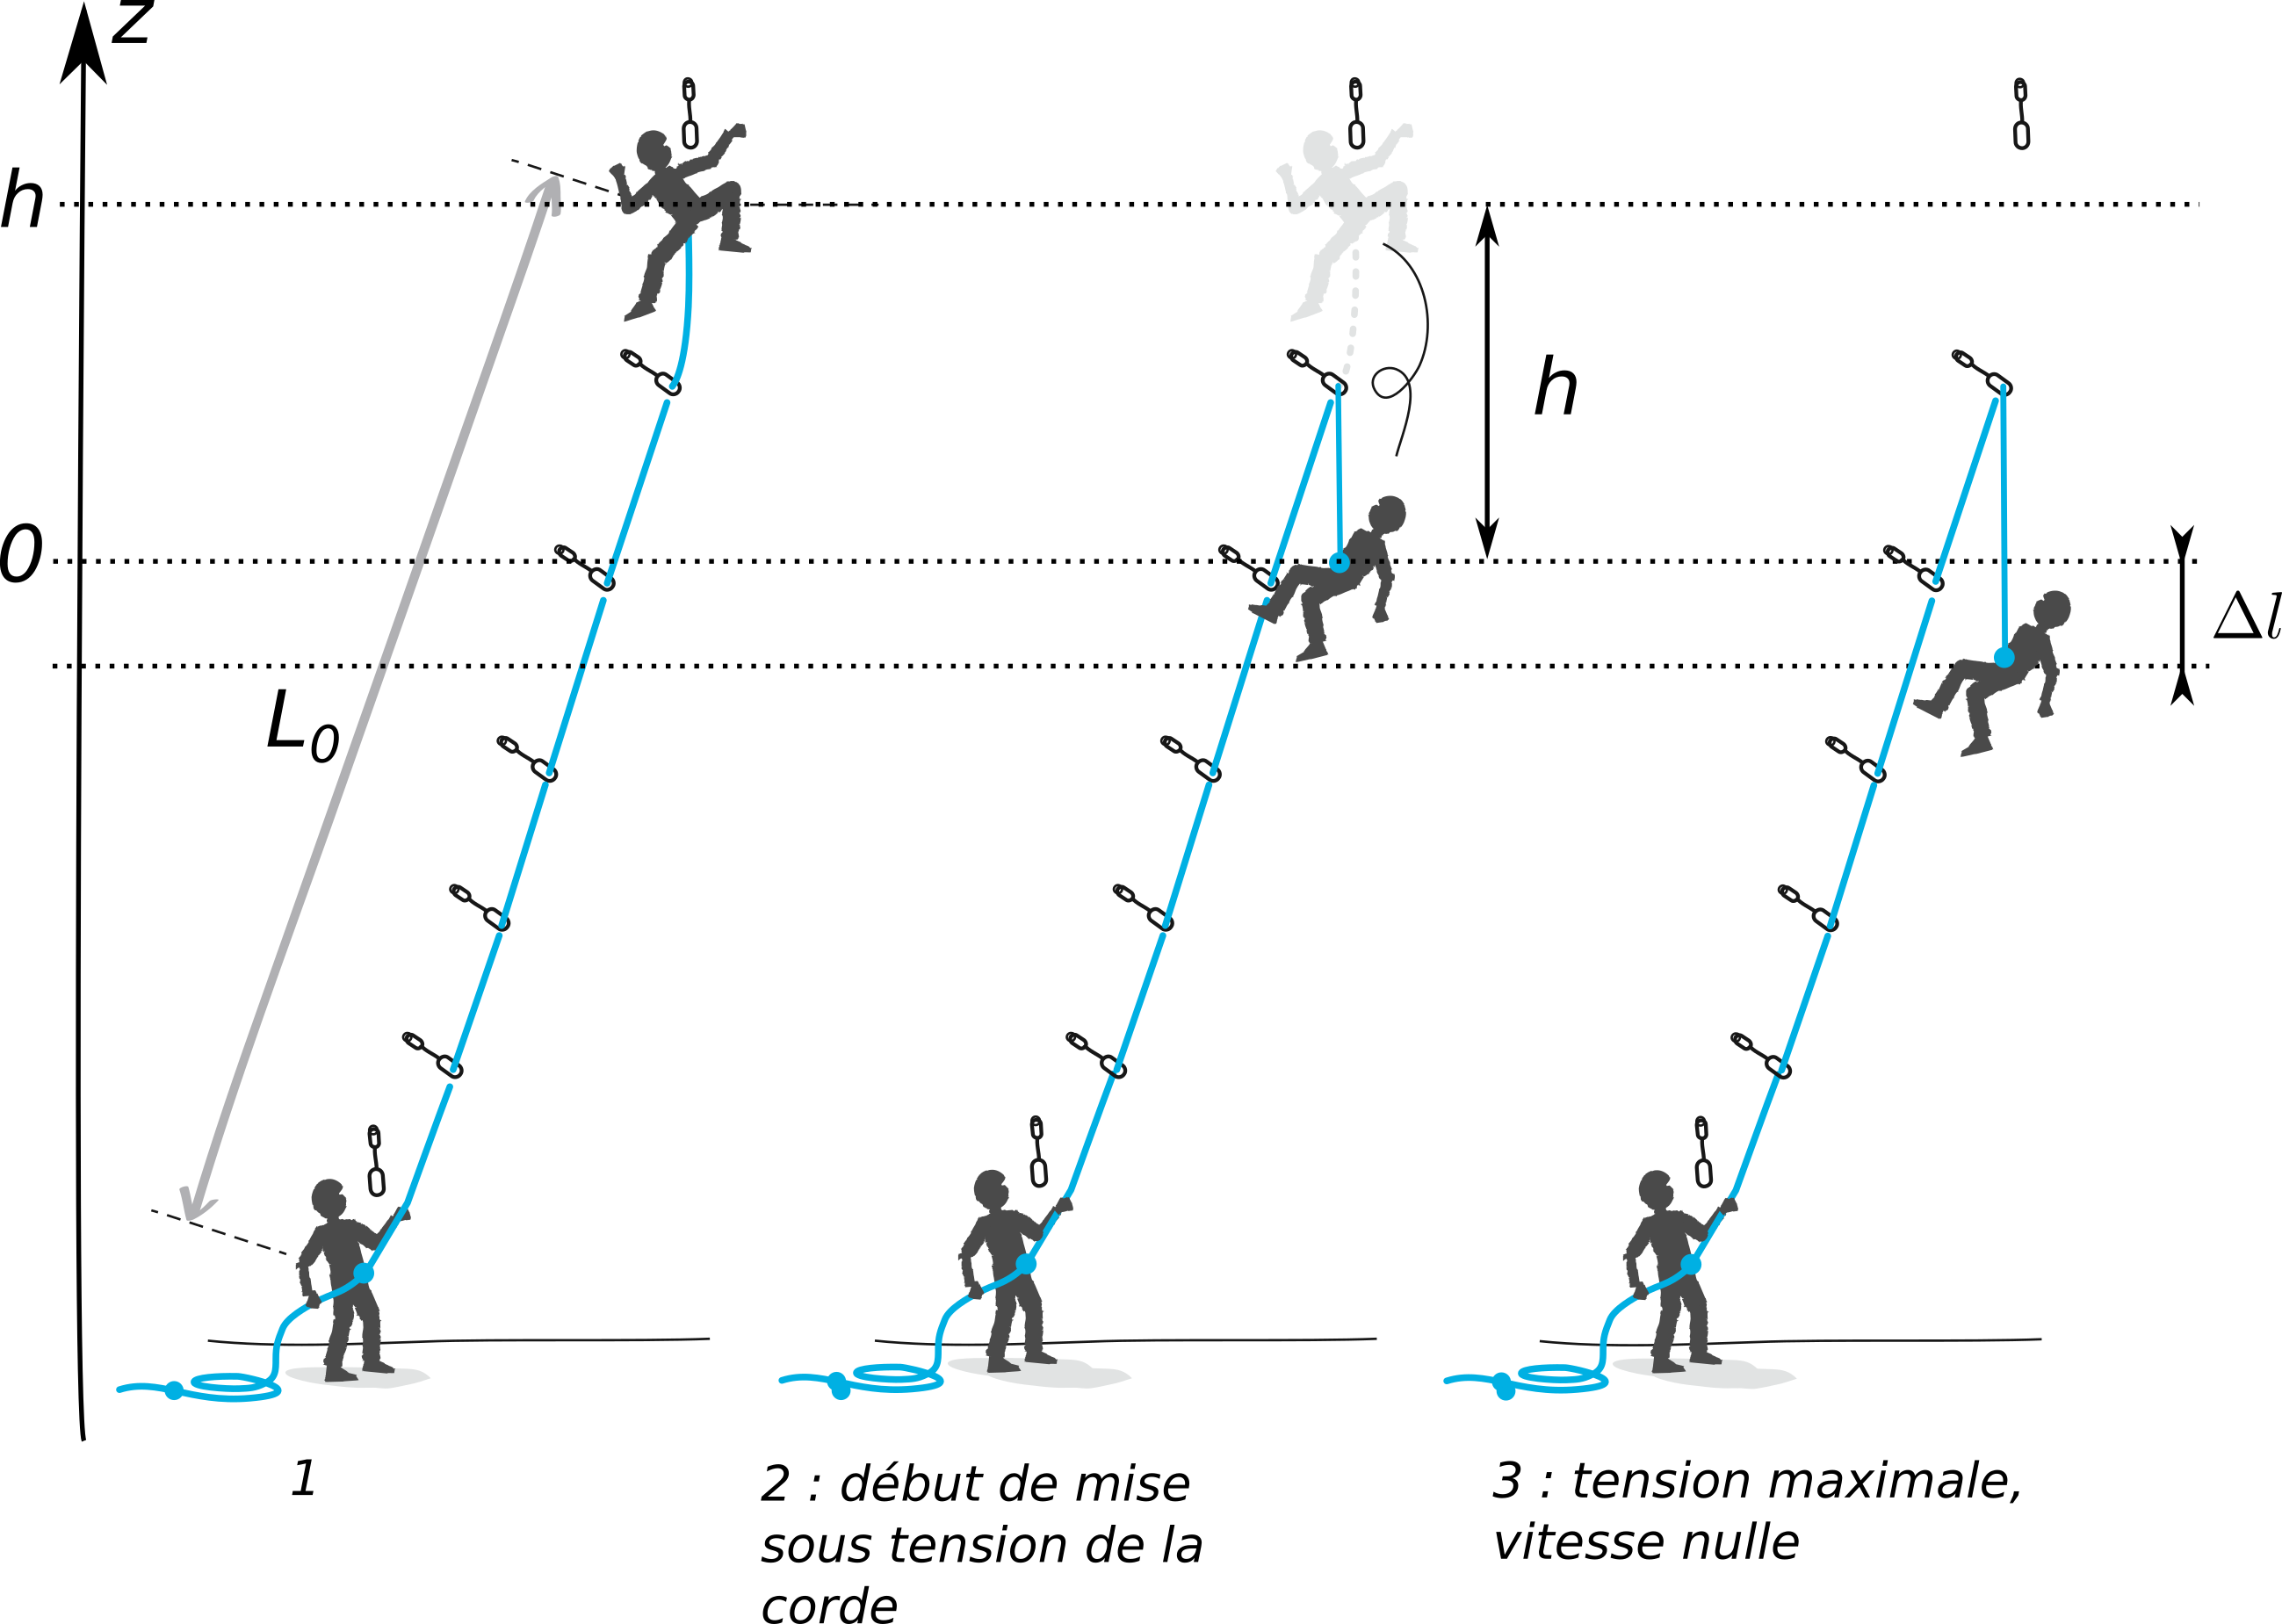
\includegraphics[width=.7\linewidth]{chute_escalade-plain}
	\end{center}

	La grimpeuse est en chute libre sur une hauteur $h$ pendant laquelle la corde
	n'est pas sous tension. La corde passe ensuite sous tension, et la chute se
	poursuit sur une hauteur $\D l$. La vitesse de la grimpeuse devient ainsi nulle
	au bout d'une hauteur totale de chute $h+\D l$.

	On prendra $g = \SI{10}{m.s^{-2}}$, $\a = \SI{5.0e4}{N}$ et une grimpeuse de
	masse $m = \SI{50}{kg}$.
}

\QR{%
	À l'aide d'un bilan énergétique, donner l'expression de la vitesse
	maximale atteinte par la grimpeuse. Faire l'application numérique pour
	une hauteur de chute $h = \SI{5}{m}$.
}{%
	Pendant la chute libre, la grimpeuse ne subit que l'action du poids,
	qui est conservatif. On peut donc utiliser le TEM, avec~:
	\begin{itemize}[label=$\diamond$]
		\litem{Au début de la chute libre~:} $z = h$, $v=0 \Ra \Ec_{p,p} = mgh$ et
		$\Ec_c = 0$
		\litem{À la fin de la chute libre~:} $z = 0$, $v=v \Ra \Ec_{p,p} = 0$ et
		$\Ec_c = mv^2/2$.
	\end{itemize}
	D'où
	\begin{gather*}
		\frac{1}{2}mv^2 = mgh
		\Lra
		\boxed{v = \sqrt{2gh}}
		\qavec
		\left\{
		\begin{array}{rcl}
			g & = & \SI{10}{m.s^{-2}} \\
			h & = & \SI{5}{m}
		\end{array}
		\right.\\
		\AN
		\boxed{v = \SI{10}{m.s^{-1}}}
	\end{gather*}
}
\QR{%
	Toujours à l'aide d'une méthode énergétique, donner l'expression de
	l'allongement maximal $\D l$ de la corde. On supposera $\D l \ll h$ afin
	de simplifier le calcul.
}{%
	On peut utiliser le TEM entre le point tout en haut et le point le
	plus bas, ou entre le point O et le point le plus bas. Faisons le
	premier cas~:
	\begin{itemize}[label=$\diamond$]
		\litem{Au début de la chute libre~:} $z = h$, $v=0 \Ra \Ec_{p,p} = mgh$ et
		$\Ec_c = 0$
		\litem{À la fin de la chute amortie~:} $z = -\D l$, $v=0 \Ra \Ec_{p,p}
			= -mg\D l$, \fbox{$\Ec_{p,el} = k\D l^2/2$} et $\Ec_c = 0$.
	\end{itemize}
	Ainsi,
	\begin{gather*}
		mgh = \frac{1}{2}k\D l^2 + mg(-\D l)
		\Lra
		mg(h+\underbracket[1pt]{\cancel{\D l}}_{\ll h}) = \frac{1}{2}k\D l^2
		\Lra
		\boxed{\D l = \sqrt{\frac{2mgh}{k}}}
		\qed
	\end{gather*}
	La solution trouvée est plausible~: homogène, augmente avec $m$, $h$ et
	$g$ mais diminue avec $k$.
}
\QR{%
	Donner enfin l'expression de la norme de la force maximal $F_{\max}$
	qu'exerce la corde sur la grimpeuse. On introduira le facteur de chute
	$f = h/L_0$.
}{%
	En norme, une force de rappel s'exprime $F = k(\ell -\ell_0)$, soit
	ici
	\begin{gather*}
		F_{\max} = k\D l = \sqrt{2mgh\,k} = \sqrt{2mgh\frac{\a}{L_0}}
		\\\Lra
		\boxed{F_{\max} = \sqrt{2mg\a f}}
		\qed
	\end{gather*}
}
\QR{%
	Au-delà d'une force de \SI{12}{kN}, les dommages sur le corps humain
	deviennent importants. Que vaut $F_{\max}$ pour une chute de $h =
		\SI{4}{m}$ sur une corde de longueur $L_0 = \SI{4}{m}$~? Conclure.
}{%
	On fait l'application numérique~:
	\begin{gather*}
		\qavec
		\left\{
		\begin{array}{rcl}
			m  & = & \SI{50}{kg}       \\
			g  & = & \SI{10}{m.s^{-2}} \\
			\a & = & \SI{5.0e4}{N}     \\
			f  & = & \num{1}
		\end{array}
		\right.\\
		\AN
		\boxed{F_{\max} = \SI{10}{kN}}
	\end{gather*}
	Il n'y a donc pas de risque aggravé pour la grimpeuse avec cette chute.
}
\QR{%
	Une chute d'un mètre arrêtée par une corde de \SI{50}{cm} est-elle
	plus ou moins dangereuse qu'une chute de \SI{4}{m} arrêtée par une corde
	de \SI{8}{m}~?
}{%
	Dans le premier cas, $f_1 = 2$~; dans le second, $f_2 = \num{0.5}$. Or,
	$F_{\max}$ évolue en $\sqrt{f}$, donc plus $f$ augmente plus la force
	subie augmente~: le premier cas est donc 2 fois plus dangereux que le
	premier~!
}

\resetQ
\section{Pendule électrique}
\enonce{%
	On étudie un pendule constitué d'une boule de polystyrène expansé recouverte
	d'une feuille d'aluminium, et suspendue à une potence par une fine tige de
	longueur $R = \SI{10}{cm}$ dont nous négligerons la masse. La boule de masse $m
		= \SI{20}{g}$ sera assimilée à un point matériel M.
	\smallbreak
	Une boule identique est placée en A (voir schéma). Les deux boules sont
	chargées électriquement avec la même charge, et donc se repoussent. La force
	exercée par A sur M s'écrit
	\[
		\Ff_e = \frac{k}{\rm AM^3} \vv{\rm AM}
		\qavec
		k = \SI{4.4e-3}{N.m^2}
	\]
	\bigbreak
	\noindent
	\begin{minipage}{0.45\linewidth}
		\begin{center}
			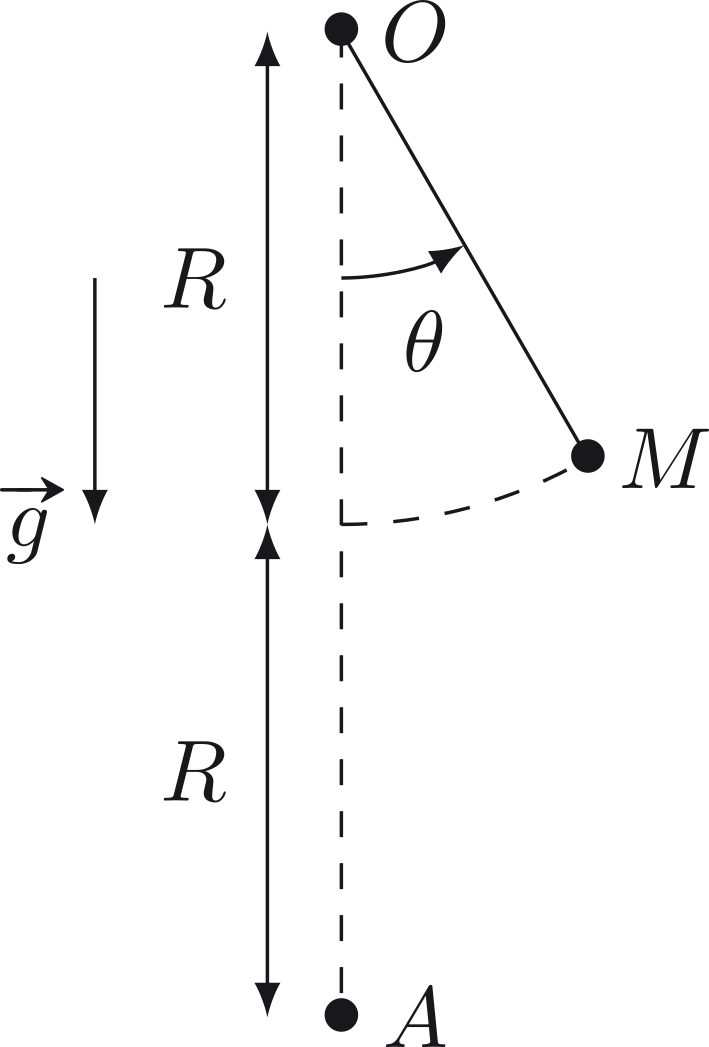
\includegraphics[height=4cm]{pendule_elec_sch-plain}
			\captionof{figure}{Dispositif}
		\end{center}
	\end{minipage}
	\hfill
	\begin{minipage}{0.35\linewidth}
		\begin{center}
			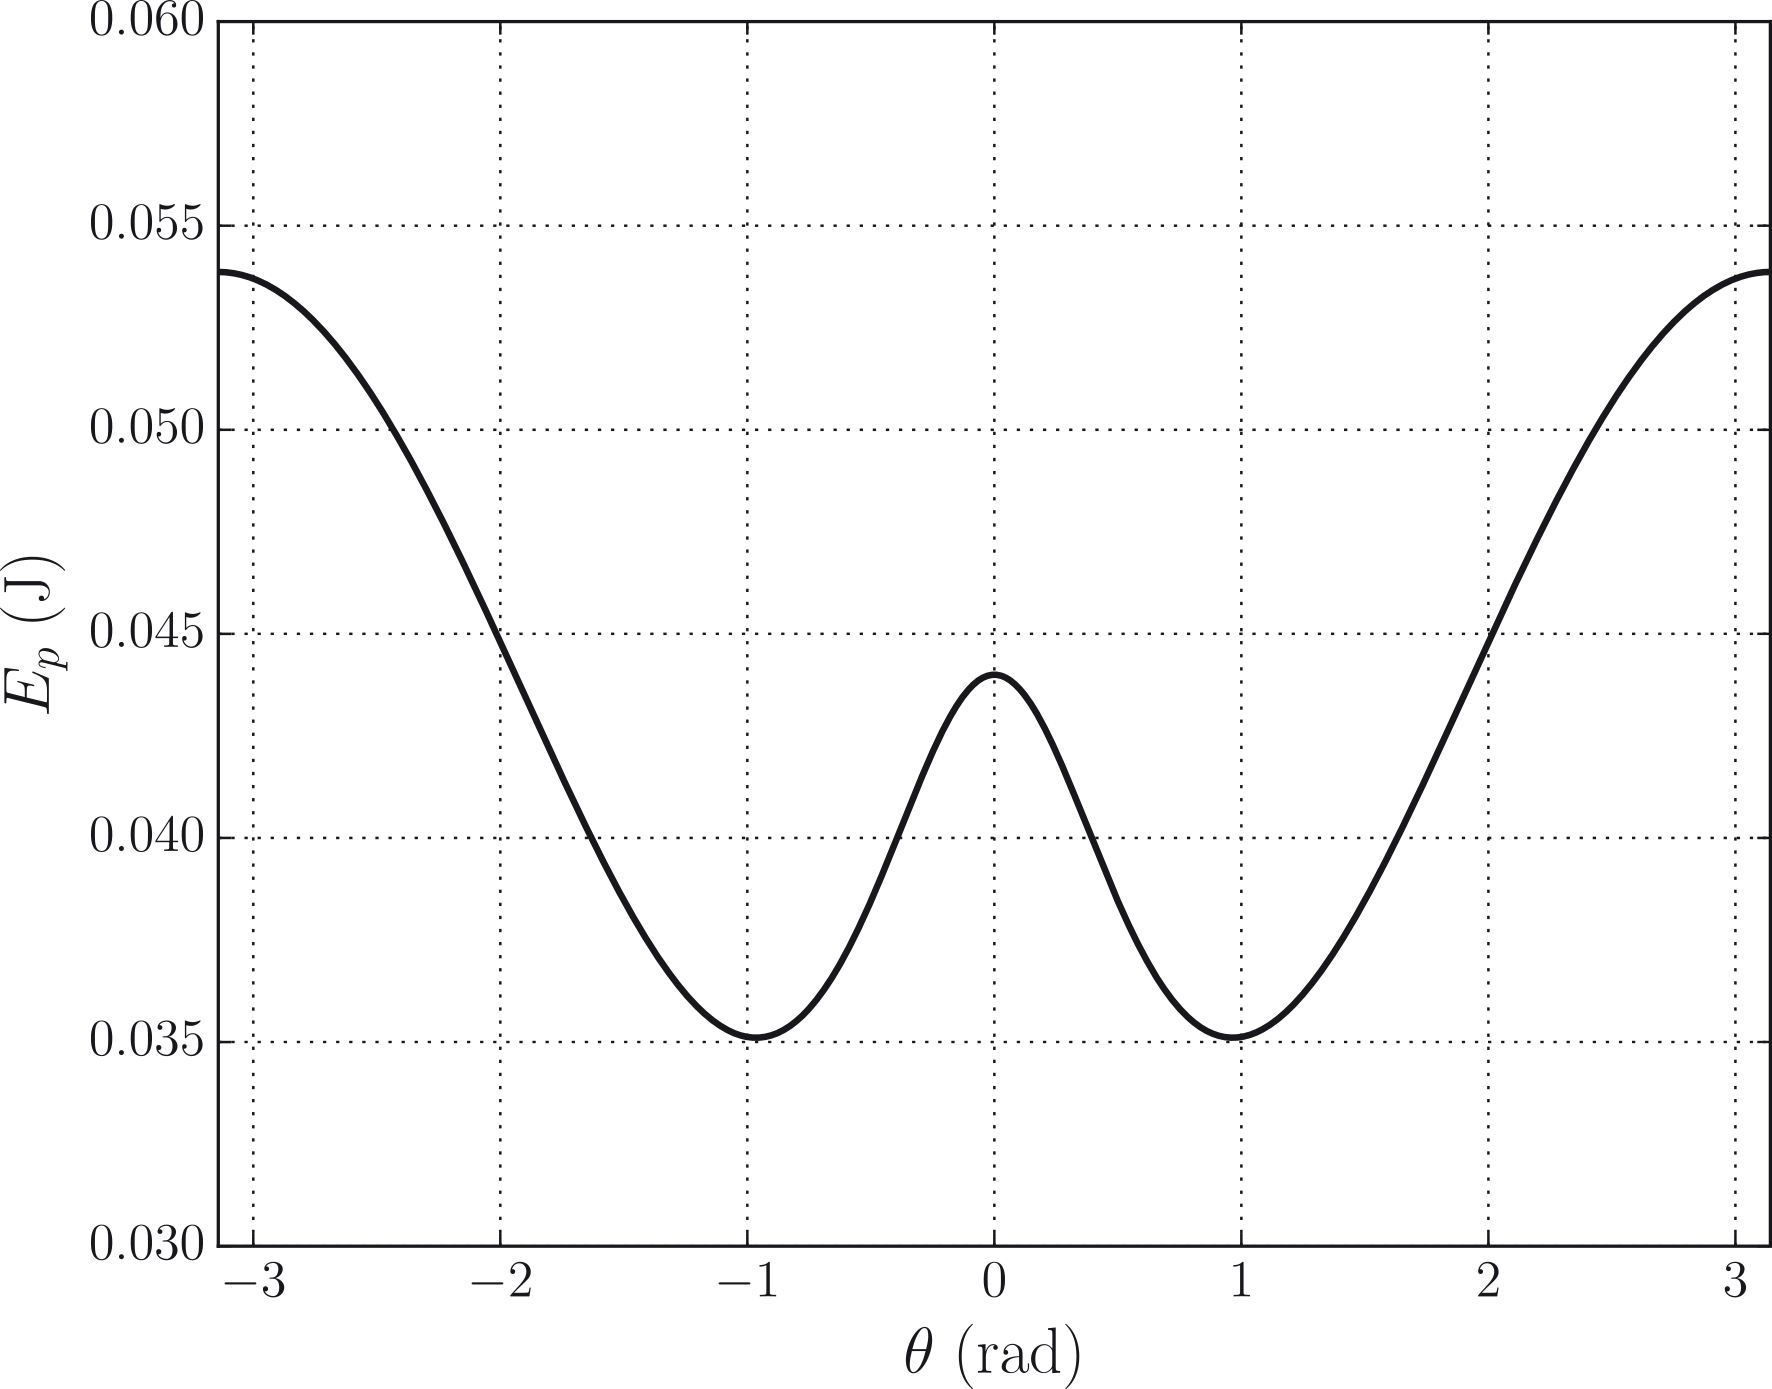
\includegraphics[width=\linewidth]{pendule_elec_ep-plain}
			\captionof{figure}{Courbe $\Ec_p(\tt)$}
		\end{center}
	\end{minipage}
}
\QR{%
	Exprimer la distance AM en fonction de $R$ et $\tt$.
}{%
	Pour exprimer la distance AM, on la décompose par des vecteurs connus
	et on pourra prendre la norme du vecteur $\vv{\rm AM}$ avec
	$\sqrt{x_{\rm AM}{}^2 + y_{\rm AM}{}^2}$, ou $\sqrt{\vv{\rm
				AM}\cdot\vv{\rm AM}}$. Notamment, $\vv{\rm AM} = \vv{\rm AO} + \OM$.
	\begin{minipage}[t]{0.33\linewidth}
		~%\vspace{-24pt}
		\begin{center}
			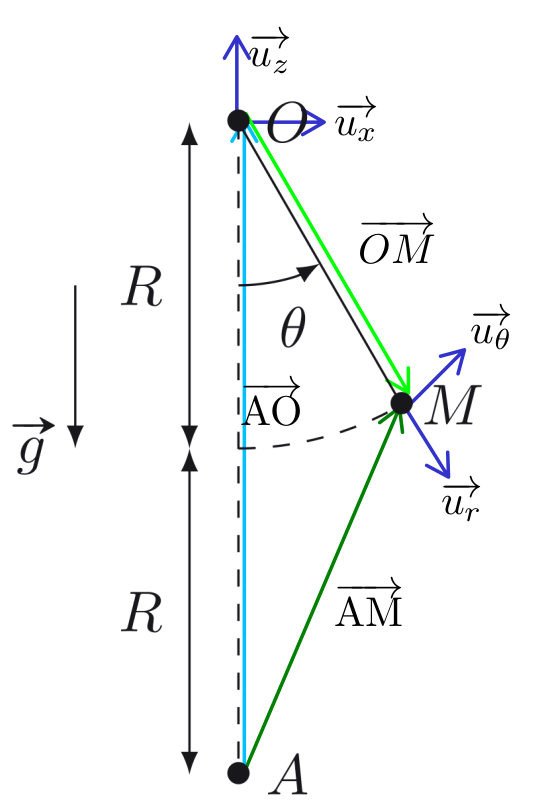
\includegraphics[width=\linewidth]{pendule_elec_am}
			\captionsetup{justification=centering}
			\captionof{figure}{Détermination de AM}
			\label{fig:pendule_am}
		\end{center}
	\end{minipage}
	\hfill
	\begin{minipage}[t]{0.65\linewidth}
		Il faut donc décomposer $\vv{\rm AO}$ et $\OM$ sur la même base,
		comme on le fait pour le poids sur un plan incliné. En effet,
		\begin{align*}
			\vv{\rm AO} & = 2R\uz \\
			\OM         & = R\ur
		\end{align*}
		mais on ne peut pas sommer les deux dans des bases différentes.
		Décomposons $\ur$ sur $(\ux, \uz)$~: on trouve
		\[\ur = \sin\tt\ux -\cos\tt\uz\]
		Ainsi,\vspace{-24pt}
		\begin{align*}
			\vv{\rm AM}        & = \vv{\rm AO} + \OM
			\\\Lra
			\vv{\rm AM}        & = \mqty(R\sin\tt                                        \\2R-R\cos\tt)
			\\\Ra
			\norm{\vv{\rm AM}} & = \sqrt{R^2\sin^2\tt + (2R-R\cos\tt)^2}
			\\\Lra
			{\rm AM}           & = \sqrt{R^2\sin^2\tt + 4R^2 -2R^2\cos\tt +R^2\cos^2\tt}
			\\\Lra
			{\rm AM}           & = \sqrt{5R^2 -2R^2\cos\tt}
			\qavec
			\cos^2\tt + \sin^2\tt = 1
			\\\Lra
			\Aboxed{{\rm AM}   & = R\sqrt{5-2\cos\tt}}
			\qed
		\end{align*}
	\end{minipage}
}
\QR{%
	Montrer que la force $\Ff_e$ est conservative, et que son énergie
	potentielle s'exprime
	\[\Ec_{p,e}(\tt) = \frac{k}{R\sqrt{5-4\cos\tt}}\]
}{%
	Une force est conservative si son travail élémentaire s'exprime sous
	la forme $-\dd\Ec_p$. Calculons son travail élémentaire~:
	\begin{align*}
		\de W(\Ff_e)         & = \Ff_e\cdot\dd{\vv{\rm AM}}
		\\\Lra
		\de W(\Ff_e)         & = \frac{k}{\rm AM^3}{\vv{\rm AM}}\cdot\dd{\vv{\rm AM}}
		\\\Lra
		\de W(\Ff_e)         & = \frac{k}{\rm AM^3} \underbracket[1pt]{\norm{\vv{\rm
					AM}}}_{=\rm AM} \norm{\dd{\vv{\rm AM}}}
		\underbracket[1pt]{\cos(\vv{\rm AM}, \dd{\vv{\rm AM}})}_{=1}
		\\\Lra
		\de W(\Ff_e)         & = \frac{k}{\rm AM^2} \cancel{\underbracket[1pt]{\frac{\rm
					AM}{\rm AM}}_{=1}} \dd{\rm AM}
		\\\Lra
		\de W(\Ff_e)         & = -k\dd(\frac{1}{\rm AM})
		\\\Lra
		\Aboxed{\de W(\Ff_e) & = -\dd{\Ec_{p,e}}}
		\\\qavec
		\Aboxed{\Ec_{p,e}    & = \frac{k}{\rm AM} = \frac{k}{R\sqrt{5-4\cos\tt}}}
		\qed
	\end{align*}
}
\QR{%
	Exprimer l'énergie potentielle totale $\Ec_p(\tt)$ de la boule M.
}{%
	La boule M a également une énergie potentielle de pesanteur. En
	prenant O comme origine de l'altitude, l'altitude de la boule M $z(\tt)$
	s'exprime
	\[z(\tt) = -R\cos\tt\]
	Ainsi,
	\begin{align*}
		\Ec_p(\tt)         & = \Ec_{p,p}(\tt) + \Ec_{p,e}(\tt)
		\\\Lra
		\Aboxed{\Ec_p(\tt) & = \frac{k}{R\sqrt{5-4\cos\tt}} - mgR\cos\tt}
		\qed
	\end{align*}
}
\QR{%
	Le tracé de l'énergie potentielle est proposé sur la figure 2. Déduire
	de ce graphe l'existence de positions d'équilibres, et indiquer leur
	nature.
}{%
	On observe en tout 5 positions d'équilibres~: deux stables dans les
	puits de potentiel vers $\pm\SI{1}{rad}$, et trois instables (maxima
	locaux d'énergie potentielle) en $-\pi$, $0$ et $\pi$.
}
\QR{%
	Discuter de la nature de la trajectoire de M suivant la valeur de son
	énergie mécanique.
}{%
	Le mouvement du pendule ne se fait que dans les zones du graphique où
	$\Ec_p < \Ec_m$. On distingue donc 4 cas~:
	\[
		\begin{array}{lrcll}
			\textbf{Cas 1} & \quad \SI{0}{J}      & < \Ec_m & < \SI{3.5e-2}{J} & \Ra
			\text{pas de mouvement}
			\\
			\textbf{Cas 2} & \quad \SI{3.5e-2}{J} & < \Ec_m & < \SI{4.4e-2}{J} & \Ra
			\text{oscillations $\approx$ position stable}
			\\
			\textbf{Cas 3} & \quad \SI{4.4e-2}{J} & < \Ec_m & < \SI{5.4e-2}{J} & \Ra
			\text{mouvement périodique entre $\Ec_{p,\max}$}
			\\
			\textbf{Cas 4} & \quad \SI{5.4e-2}{J} & < \Ec_m & < +\infty        & \Ra
			\text{mouvement révolutif~: tours à l'infini}
		\end{array}
	\]
	\begin{center}
		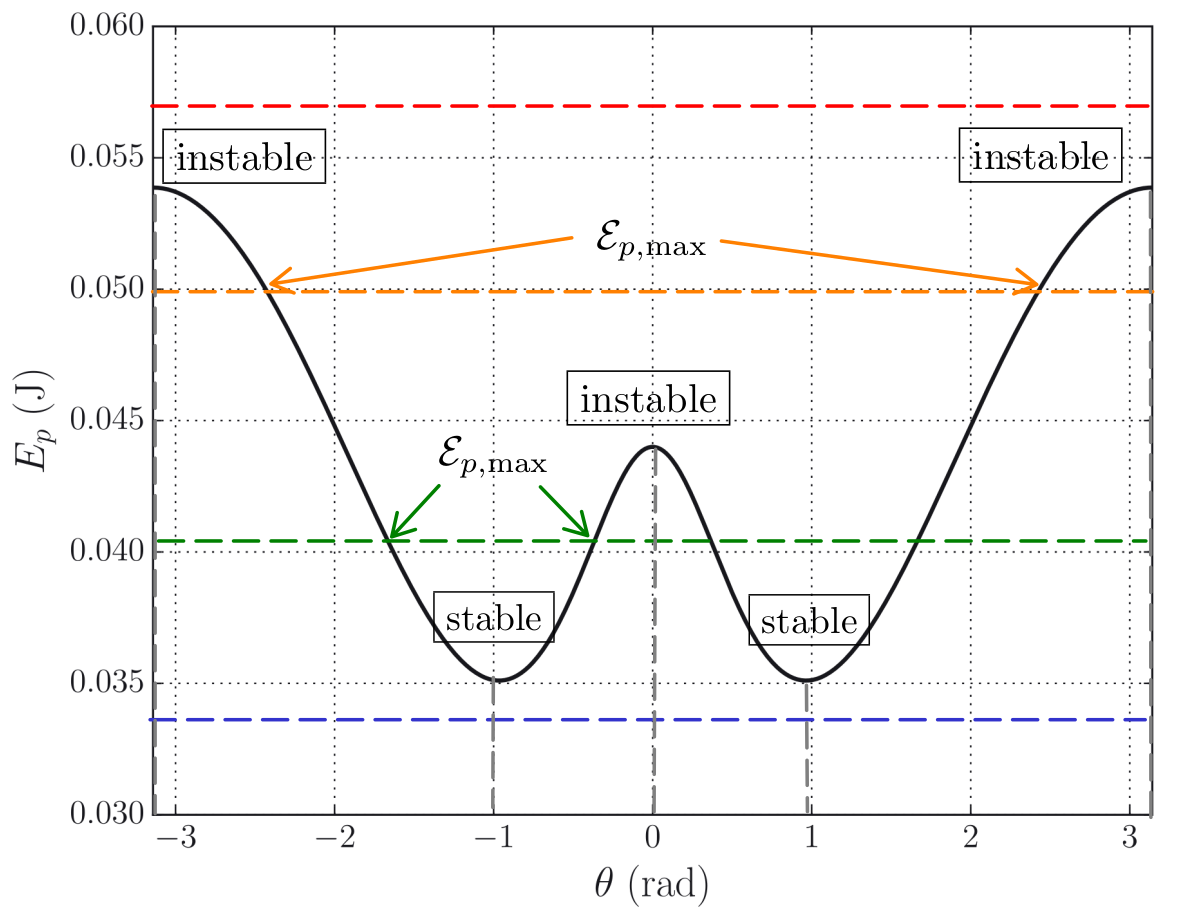
\includegraphics[width=.7\linewidth]{pendule_elec_ep_corr}
		\captionof{figure}{Mouvement selon $\Ec_m$}
		\label{fig:pend_elec_em}
	\end{center}
}

\resetQ
\section{Recul d'un canon}
\enonce{%
	On considère un canon (figure~\ref{fig:canon}) de masse $M = \SI{800}{kg}$. Lors
	du tir horizontal d'un obus de masse $m = \SI{2.0}{kg}$ avec une vitesse
	$\vfo=v_0\ux$ telle que $v_0 = \SI{600}{m.s^{-1}}$, le canon acquiert une
	vitesse de recul $\vv{v_c} = -\frac{m}{M}\vfo$.

	Pour limiter la course du canon, on utilise un ressort de raideur $k_1$, de
	longueur à vide $L_0$ dont l'une des extrémités est fixe, et l'autre liée au
	canon. Le déplacement a lieu suivant l'axe O$x$. Dans la suite, le canon est
	assimilé à un point matériel, son centre de gravité G (figure~\ref{fig:rep}).

	\begin{minipage}{0.40\linewidth}
		\begin{center}
			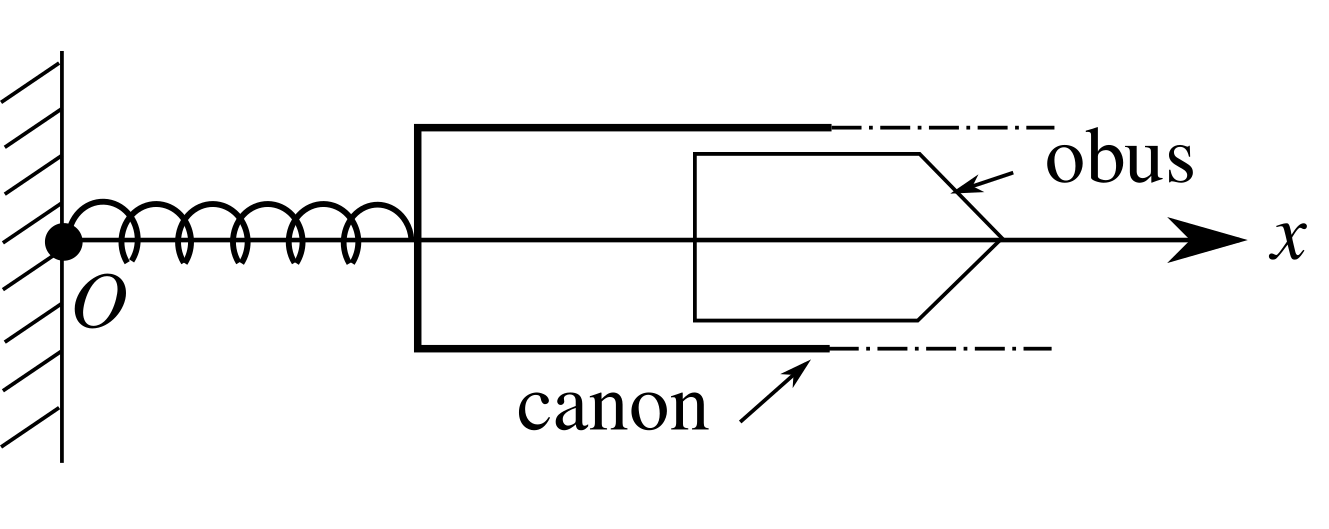
\includegraphics[height=3cm]{recul_canon_a-plain}
			\captionof{figure}{Canon}
			\label{fig:canon}
		\end{center}
	\end{minipage}
	\hfill
	\begin{minipage}{0.23\linewidth}
		\begin{center}
			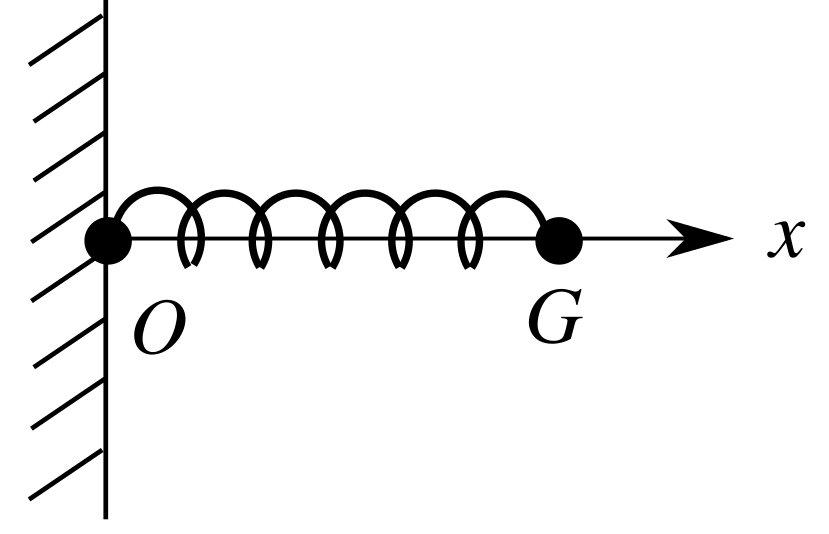
\includegraphics[height=3cm]{recul_canon_b-plain}
			\captionof{figure}{Repérage}
			\label{fig:rep}
		\end{center}
	\end{minipage}
	\hfill
	\begin{minipage}{0.31\linewidth}
		\begin{center}
			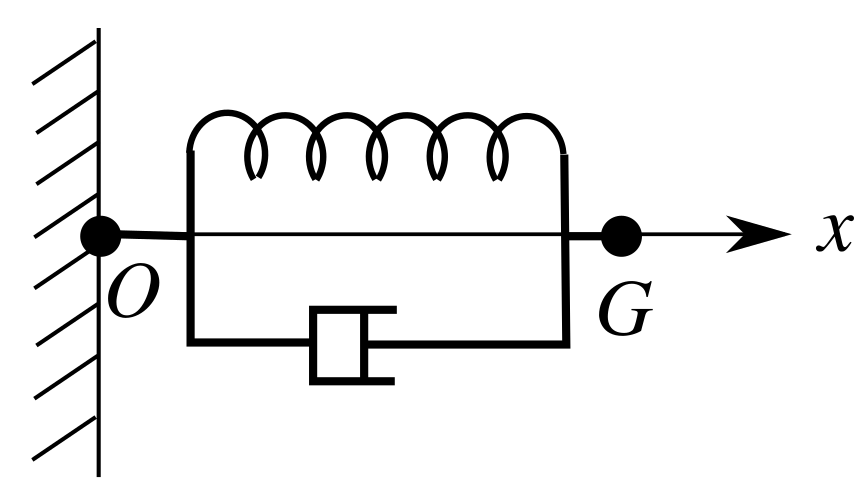
\includegraphics[height=3cm]{recul_canon_c-plain}
			\captionof{figure}{Amortisseur}
			\label{fig:amor}
		\end{center}
	\end{minipage}
}

\QR{%
	Quelle est la longueur du ressort lorsque le canon est au repos~?
}{%
	Au repos, la tension du ressort est nulle, donc $\ell = L_0$.
}
\QR{%
	En utilisant l'énergie mécanique, déterminer la distance de recul $d$.
	En déduire la raideur $k_1$ pour avoir un recul inférieur ou égal à $d$.
	Application numérique pour $d = \SI{1.0}{m}$.
}{%
	\begin{itemize}[label=$\diamond$, leftmargin=10pt]
		\litem{Système~:} \{canon\}, repéré par G de masse $M$
		\litem{Référentiel~:} $\Rc\ind{sol}$, supposé galiléen
		\litem{Repère~:} mouvement horizontal donc cartésien, $(\Or,\ux,\uz)$
		avec $\uz$ vertical ascendant
		\litem{Repérage~:}
		\begin{align*}
			\OG & = x\ux    \\
			\vf & = \xp\ux  \\
			\af & = \xpp\ux
		\end{align*}
		\litem{BDF~:}
		\[
			\begin{array}{ll}
				\textbf{Poids}    & \Pf = -mg\uz         \\
				\textbf{Réaction} & \Nf = N\uz           \\
				\textbf{Ressort}  & \Ff = -k_1(x-L_0)\ux
			\end{array}
		\]
		Le poids et la tension du ressort sont conservatives, et la
		réaction du sol ne travaille pas~: on a donc un système
		conservatif, et on applique simplement le TEM~:
		\litem{Au moment du tir~:} $v=v_c$, $x=L_0 \Ra \Ec_{c,0} =
			Mv_c{}^2/2$ et $\Ec_{p,el} = k_1(L_0-L_0)^2/2 = 0$
		\litem{Après le recul~:} $v=0$, $x=L_0-d \Ra \Ec_{c,f} = 0$ et
		$\Ec_{p, el} = k_1d^2/2$
		\litem{TEM~:}
		\begin{align*}
			\frac{1}{2}k_1d^2 & =
			\frac{1}{2}M\underbracket[1pt]{v_c}_{\mathclap{=mv_0/M}}{}^2
			\\\Lra
			d^2               & = \frac{m^2}{k_1M}v_0{}^2
			\\\Lra\,
			\Aboxed{d         & = \frac{m}{\sqrt{k_1M}}v_0}
			\qed
			\\\Lra\,
			\Aboxed{k_1       & = \frac{m^2v_0{}^2}{d^2M}}
			\qed
			\qavec
			\left\{
			\begin{array}{rcl}
				m   & = & \SI{2.0}{kg}       \\
				M   & = & \SI{800}{kg}       \\
				v_0 & = & \SI{600}{m.s^{-1}} \\
				d   & = & \SI{1.0}{m}
			\end{array}
			\right.                                         \\
			\AN
			\Aboxed{k_1       & = \SI{1800}{N.m^{-1}}}
		\end{align*}
	\end{itemize}
}
\QR{%
	Retrouver la relation entre $k_1$ et $d$ en appliquant le PFD.
}{%
	Avec le \textbf{PFD} et en projetant sur $\ux$ (on a $N = mg$ sur
	$\uz$)~:
	\begin{align*}
		M\xpp            & = -k_1(x-L_0)
		\\\Lra
		\xpp + \w_0{}^2x & = \w_0{}^2L_0
		\qavec
		\w_0 = \sqrt{\frac{k_1}{M}}
		\\\Ra
		x(t)             & = A\cos(\w_0t+\f) + L_0
		\shortintertext{Or,}
		x(t=0) = L_0     & \Ra A\cos\f = 0
		\shortintertext{On choisit $\f = -\pi/2$, et ainsi}
		x(t)             & = A\sin(\w_0t) + L_0
		\\\Ra
		\xp(t)           & = A\w_0\cos(\w_0t)
		\shortintertext{Or,}
		\xp(t=0)         & = -\frac{m}{M}v_0
		\\\Ra
		A                & = -\frac{m}{M} \frac{v_0}{\w_0}
		\\\Ra
		\Aboxed{x(t) = -\frac{mv_0}{\sqrt{k_1M}}\sin(\w_0t)+L_0}
		\qed
	\end{align*}
	On obtient alors $d$ comme étant l'amplitude du sinus, c'est-à-dire le
	résultat précédent.
}
\QR{%
	Quel est l'inconvénient d'utiliser un ressort seul~?
}{%
	On vient donc de démontrer qu'avec un seul ressort, le canon va
	osciller et donc après le recul, il va repartir vers l'avant.
	L'amplitude va diminuer petit à petit à cause des frottements
	inéluctables, mais le temps avant immobilisation sera important~: on a
	donc intérêt à ajouter une force de frottements visqueux.
}
\enonce{%
	Pour pallier ce problème, on ajoute au système un dispositif amortisseur
	(figure~\ref{fig:amor}), exerçant une force de frottement $\Ff = -\lb\vf$, $\vf$
	étant la vitesse du canon.
}

\QR{%
Le dispositif de freinage absorbe une fraction $\Ec_a = \SI{778}{J}$
de l'énergie cinétique initiale. Calculer la nouvelle valeur $k_2$ de la
constante de raideur du ressort avec les données numériques précédentes.
Déterminer la pulsation propre $\w_0$ de l'oscillateur.
}{%
Le système n'est plus conservatif, et la variation d'énergie mécanique
est maintenant égale à l'énergie absorbée par le dispositif de freinage,
c'est-à-dire
\[\D\Ec_m = \Ec_{m,f} - \Ec{m,i} = -\Ec_a\]
puisque l'énergie cinétique doit décroître et que $\Ec_a$ est positive.
Or, initialement et finalement,
\[
	\Ec_{m,i} = \Ec_c = \frac{1}{2}Mv_c{}^2
	\qet
	\Ec_{m,f} = \Ec_p = \frac{1}{2}k_2d^2
\]
Soit
\begin{align*}
	\frac{1}{2}k_2d^2 - \frac{1}{2}Mv_c{}^2 & = -\Ec_a
	\\\Lra
	k_2                                     & = \frac{1}{d^2}\left(Mv_c{}^2 -2\Ec_a\right)
	\\\Lra
	\Aboxed{k_2                             & = \frac{1}{d^2}\left(\frac{m^2}{M}v_0{}^2
		-2\Ec_a\right)}
	\qed
	\qavec
	\left\{
	\begin{array}{rcl}
		m     & = & \SI{2.0}{kg}       \\
		M     & = & \SI{800}{kg}       \\
		v_0   & = & \SI{600}{m.s^{-1}} \\
		\Ec_a & = & \SI{778}{J}
	\end{array}
	\right.                                                                                \\
	\AN
	\Aboxed{k_2                             & = \SI{244}{N.m^{-1}}}                        \\
	\text{De plus, }
	\Aboxed{\w_0                            & = \sqrt{\frac{k_2}{M}}}
	\qavec
	\left\{
	\begin{array}{rcl}
		k_2 & = & \SI{244}{N.m^{-1}} \\
		M   & = & \SI{800}{kg}
	\end{array}
	\right.                                                                                \\
	\AN
	\Aboxed{\w_0                            & = \SI{0.55}{rad.s^{-1}}}
\end{align*}
}
\QR{%
	Déterminer $\lb$ pour que le régime soit critique. Application
	numérique.
}{%
	On reprend la question 3) mais avec la force de frottements, pour
	obtenir l'équation d'un oscillateur amorti~:
	\[\xpp + \frac{\lb}{M}\xp + \w_0{}^2x = \w_0{}^2L_0\]
	Le discriminant de l'équation caractéristique associée est
	\[\D = \left( \frac{\lb}{M} \right)^2 - 4\w_0{}^2\]
	et on a un régime critique quand ce discriminant est nul~; soit
	\begin{align*}
		\Aboxed{\lb & = 2M\w_0}
		\qed
		\qavec
		\left\{
		\begin{array}{rcl}
			M    & = & \SI{800}{kg}          \\
			\w_0 & = & \SI{0.55}{rad.s^{-1}}
		\end{array}
		\right.                              \\
		\AN
		\Aboxed{\lb & = \SI{884}{kg.s^{-1}}}
	\end{align*}
}
\QR{%
	Déterminer l'expression de l'élongation $x(t)$ du ressort, ainsi que
	celle de la vitesse $\xp(t)$. En déduire l'instant $t_m$ pour lequel le
	recul est maximal. Exprimer alors ce recul en fonction de $m$, $v_0$ et
	$\lb$. L'application numérique redonne-t-elle la valeur de $d$
	précédente~?
}{%
	Avec le régime critique, on a
	\begin{align*}
		x(t)           & = (At+B)\exp(-\frac{\lb t}{2M}) + L_0
		\shortintertext{Or,}
		x(0) = 0       & \Ra \boxed{B=0}
		\\\Ra
		\xp(t)         & = A\exp(-\frac{\lb t}{2M})\left(1-\frac{\lb}{2M}t\right)
		\shortintertext{Or,}
		\xp(0) = v_c   & \Ra \boxed{A = v_c}
		\\\Ra\quad
		\Aboxed{\xp(t) & = -\frac{m}{M}\exp(-\frac{\lb t}{2M})
			\left(1-\frac{\lb}{2M}t\right)}
		\\\text{et}\quad
		\Aboxed{x(t)   & = -\frac{m}{M}v_0t\exp(-\frac{\lb t}{2M}) + L_0}
		\qed
	\end{align*}
	Le recul est maximal quand la vitesse s'annule, soit
	\begin{gather*}
		t_m = \frac{2M}{\lb} = \SI{1.8}{s}
	\end{gather*}
	On calcule $x(t_m)$, sachant qu'on a par définition $x(t_m) = L_0 - d$~:
	\begin{align*}
		x(t_m)    & = -\frac{m}{M}v_0\frac{2M}{\lb}\exr^{-1} + L_0
		\\\Lra
		L_0 - d   & = L_0 - \frac{2mv_0}{\lb \exr}
		\\\Lra
		\Aboxed{d & = \frac{2mv_0}{\lb\exr}}
		\qed
	\end{align*}
	et l'application numérique donne
	\[\boxed{d = \SI{1.0}{m}}\]
	On retrouve bien la distance de recul précédente, mais cette fois il n'y
	a pas d'oscillation~! Cahier des charges rempli.
}

\resetQ
\section{Positions d'équilibre d'un anneau sur un cercle}
\enonce{%
	\begin{minipage}{0.60\linewidth}
		Un anneau assimilable à un point matériel M de masse $m$ peut glisser sans
		frottement sur une glissière circulaire de rayon $R$ et de centre O.
		L'anneau est attaché à un ressort de raideur $k$ dont une extrémité est
		fixée à la glissière au point A. Sa position est repérée par l'angle $\tt$
		entre le rayon OM et l'axe horizontal (O$x$). Pour simplifier les calculs,
		on considérera que la longueur à vide $\ell_0$ du ressort est nulle.
	\end{minipage}
	\hfill
	\begin{minipage}{0.35\linewidth}
		\begin{center}
			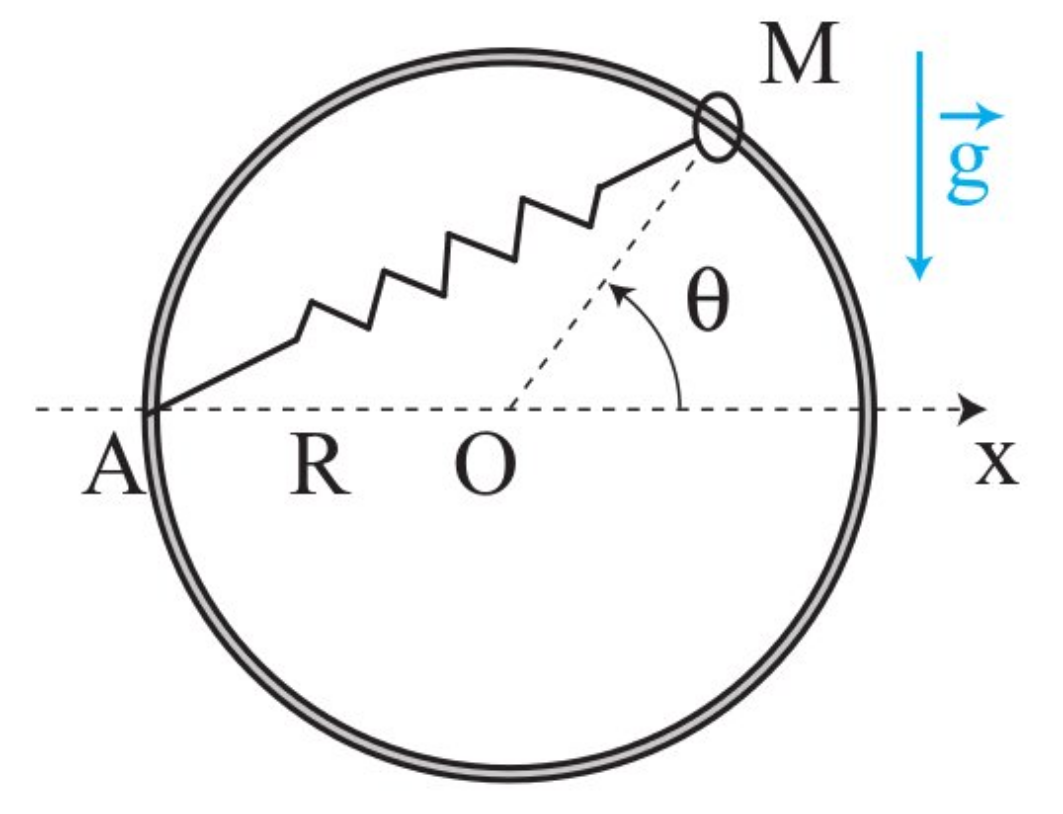
\includegraphics[width=.9\linewidth]{anneau_cercle_ressort-plain}
		\end{center}
	\end{minipage}
}

\QR{%
	Montrer que la longueur $\ell$ s'exprime $\ell = R\sqrt{2(1+\cos\tt)}$.
}{%
	\begin{minipage}[t]{0.25\linewidth}
		~
		\begin{center}
			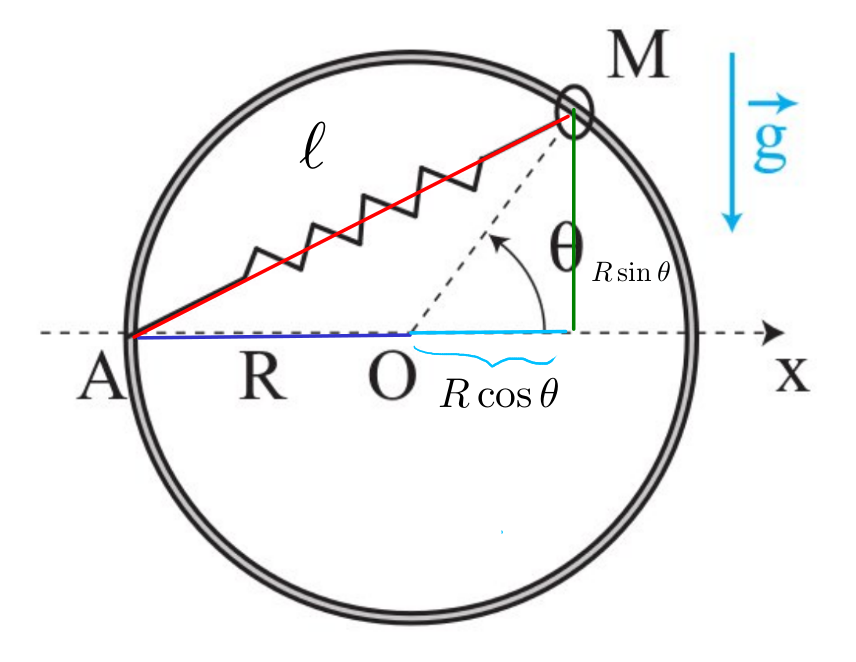
\includegraphics[width=\linewidth]{anneau_cercle_ressort-proj}
			\captionsetup{justification=centering}
			\captionof{figure}{Détermination de $\ell$}
			\label{fig:anncercproj}
		\end{center}
	\end{minipage}
	\hfill
	\begin{minipage}[t]{0.70\linewidth}
		On peut réutiliser la relation de \textsc{Chasles} pour écrire
		$\vv{\rm AM} = \vv{\rm AO} + \OM$ et déterminer la distance en prenant
		la norme, mais ici une simple utilisation du théorème de
		\textsc{Pythagore} suffit. On projette M sur l'axe $x$ pour avoir
		\begin{align*}
			\ell^2       & = (R+R\cos\tt)^2 + (R\sin\tt)^2
			\\\Lra
			\ell^2       & = R^2 + 2R^2\cos\tt + R^2(\cos^2\tt + \sin^2\tt)
			\\\Lra
			\ell^2       & = 2R^2(1+\cos\tt)
			\\\Lra
			\Aboxed{\ell & = R\sqrt{2(1+\cos\tt)}}
			\qed
		\end{align*}
	\end{minipage} \bigbreak
}
\QR{%
	Exprimer l'énergie potentielle $\Ec_p$ du système constitué de
	l'anneau et du ressort en fonction de l'angle $\tt$.
}{%
	L'énergie potentielle totale $\Ec_p$ est constituée de l'énergie
	potentielle de pesanteur de l'anneau et de l'énergie potentielle
	élastique du ressort. Pour $\Ec_{p,p}$ avec origine en O, on a une
	altitude $R\sin\tt$~; pour $\Ec_{p,el}$ on a la différence de longueur à
	a vide $\ell -\ell_0$ avec $\ell_0 = 0$, d'où
	\begin{align*}
		\Ec_p         & = \Ec_{p,p} + \Ec_{p,el}
		\\\Lra
		\Ec_p         & = mgR\sin\tt + \frac{k}{2}\ell^2
		\\\Lra
		\Aboxed{\Ec_p & = mgR\sin\tt + kR^2(1+\cos\tt)}
		\qed
	\end{align*}
}
\QR{%
	Déterminer les positions d'équilibre de l'anneau.
}{%
	On trouve les positions d'équilibre de l'anneau en trouvant les angles
	$\tt_{\eq}$ tels que la dérivée de $\Ec_p$ s'annule, soit
	\begin{align*}
		\eval{\dv{\Ec_p}{\tt}}_{\tt_{\eq}} & = -kR^2\sin\tt_{\eq} +
		mgR\cos\tt_{\eq} = 0
		\\\Lra
		\sin\tt_{\eq}                      & = \frac{mg\cancel{R}}{kR^{\cancel{2}}}\cos\tt_{\eq}
		\\\Lra
		\tan\tt_{\eq}                      & = \frac{mg}{kR}
		\\\Lra
		\boxed{\tt_{\eq,1} = \arctan(\frac{mg}{kR})}
		\quad                              & \text{et}\quad
		\boxed{\tt_{\eq,2} = \pi + \arctan(\frac{mg}{kR})}
		\qed
	\end{align*}
	avec $\tt_{\eq,1}$ compris entre 0 et \ang{90}, et $\tt_{\eq,2}$ compris
	entre 180 et \ang{270}.
}
\QR{%
	Préciser si les positions d'équilibre obtenues sont stables.
}{%
	On étudie la stabilité des positions en évaluant la dérivée seconde de
	$\Ec_p$ en ce point et en vérifiant son signe. On obtient
	\begin{align*}
		\eval{\dv[2]{\Ec_p}{\tt}}_{\tt_{\eq}} & = -kR^2\cos\tt_{\eq}
		-mgR\sin\tt_{\eq}
		\\\Lra
		\eval{\dv[2]{\Ec_p}{\tt}}_{\tt_{\eq}} & = -\left(kR^2 +
		\frac{m^2g^2}{k}\right)\cos\tt_{\eq}
	\end{align*}
	en utilisant les résultats précédents sur la dérivée première de
	$\Ec_p$. L'intérieur de la parenthèse étant positif, le signe de cette
	dérivée seconde est opposé à celui du cosinus de la position
	d'équilibre. Or,
	$\cos\tt_{\eq,1} > 0$ et $\cos\tt_{\eq,2} < 0$, donc
	\begin{gather*}
		\boxed{\eval{\dv[2]{\Ec_p}{\tt}}_{\tt_{\eq,1}} < 0}
		\qet
		\boxed{\eval{\dv[2]{\Ec_p}{\tt}}_{\tt_{\eq,2}} > 0}
		\qed
	\end{gather*}
	La première position est donc instable, et la seconde stable.
}
\begin{figure}[htbp]
	\centering
	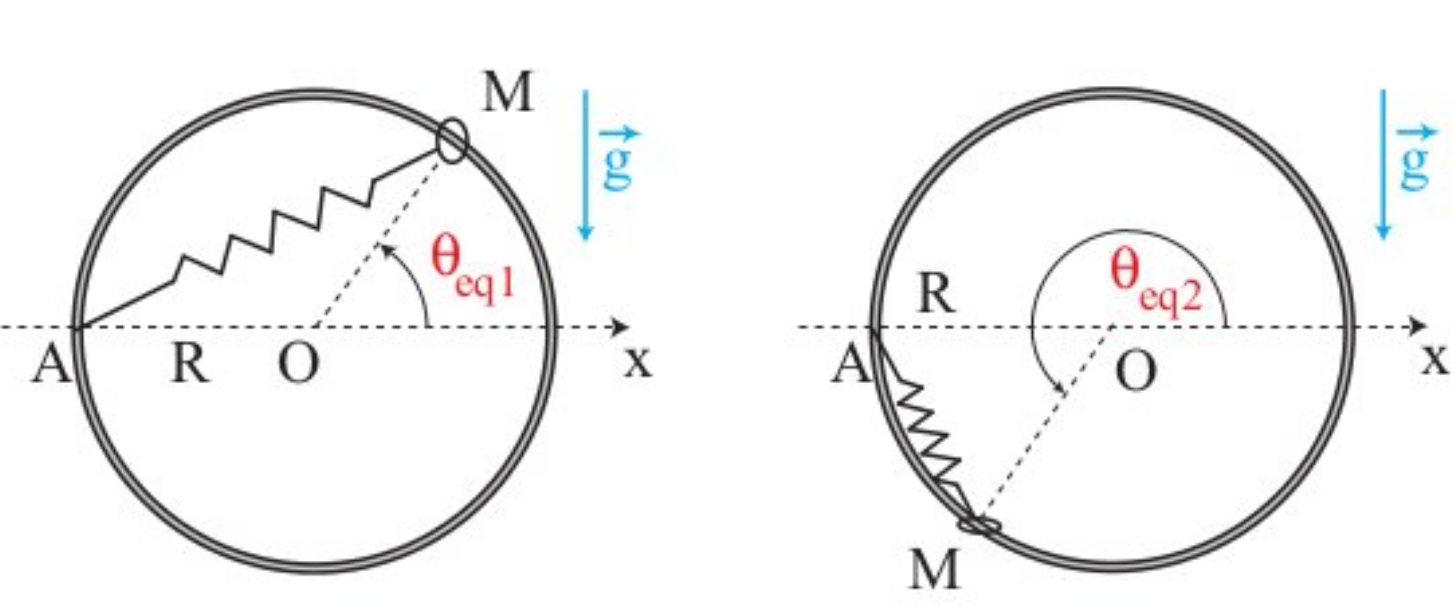
\includegraphics[width=.5\linewidth]{anneau_cercle_ressort-corr_eq}
	\captionsetup{justification=centering}
	\caption{Positions d'équilibre du système}
	\label{fig:anncerccorr}
\end{figure}

\resetQ
\section{Oscillateur de \textsc{Landau}}

\enonce{%
	L'oscillateur de \textsc{Landau} est un modèle théorique permettant de modéliser
	efficacement des systèmes physiques pour lesquelles des faibles non-linéarités
	sont à prendre en compte. Il s'agit d'une approximation un peu plus précise que
	celle de l'oscillateur harmonique pour étudier le comportement de systèmes au
	voisinage de leur position d'équilibre.
	\bigbreak
	\noindent
	\begin{minipage}{0.70\linewidth}
		Un exemple de système modèle permettant de réaliser un oscillateur de Landau
		est un petit anneau, assimilé à un point matériel M de masse $m$, astreint à
		se déplacer sans frottement le long d'une tige rectiligne horizontale
		choisie comme axe (O$x$). Cet anneau est relié à un ressort, de longueur à
		vide $\ell_0$ et de raideur $k$, dont l'autre extrémité est fixée en A. La
		distance de A à la tige est notée ${\rm AO} = a$.
	\end{minipage}
	\hfill
	\begin{minipage}{0.25\linewidth}
		\begin{center}
			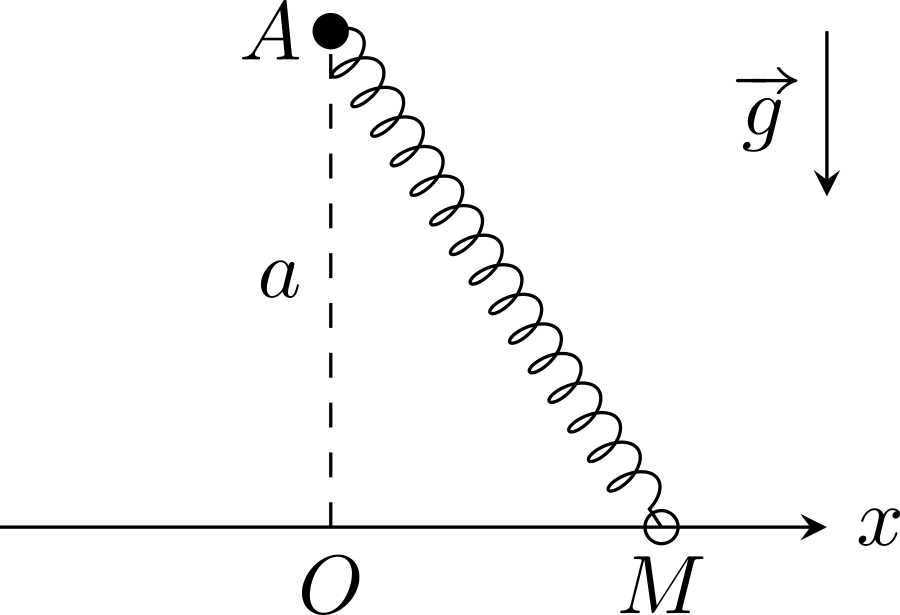
\includegraphics[width=\linewidth]{landeau_sch-plain}
		\end{center}
	\end{minipage}
}

\QR{%
	Exprimer l'énergie potentielle totale $\Ec_p(x)$.
}{%
	Comme l'anneau est contraint de se déplacer sur une ligne horizontale,
	son énergie potentielle de pesanteur est constante. Ainsi, la seule
	contribution à l'énergie potentielle est d'origine élastique,
	\[\Ec_p(x) = \frac{1}{2}k({\rm AM} -\ell_0)^2\]
	La longueur AM s'exprime à partir du théorème de \textsc{Pythagore},
	\[
		{\rm AM}^2 = a^2 + x^2
		\quad\text{d'où}\quad
		\boxed{\Ec_p(x) = \frac{1}{2}k\left(\sqrt{a^2+x^2} - \ell_0\right)^2}
	\]
}
\QR{%
	La courbe d'énergie potentielle est représentée ci-dessous pour quatre
	valeurs de $a$~: $a_1 = \ell_0/10$, $a_2 = \ell_0/3$, $a_3 = \ell_0$ et
	$a_4 = 3\ell_0$. En raisonnement qualitativement sur les positions
	d'équilibre, attribuer chaque courbe à la valeur de $a$ qui lui
	correspond.
}{%
	Qualitativement, il est assez simple de comprendre pourquoi certaines
	courbes font apparaître deux minima et d'autre un seul. Si $a < \ell_0$,
	alors deux positions de M, symétriques par rapport à O sont telles que
	${\rm AM} = \ell_0$. Dans ce cas, l'énergie potentielle élastique est
	nulle. Au contraire, si $a > \ell_0$, le ressort est toujours étiré et
	l'énergie potentielle élastique jamais nulle.
	\begin{bexem}{}
		\bfseries Ce raisonnement se retrouve tout à fait sur l'expression
		mathématique de $\Ec_p$~!
	\end{bexem}
	Ainsi on peut identifier la courbe en \textbf{pointillés violets au cas
		$\mathbf{a_4 = 3\ell_0}$}. La courbe en \textbf{points verts} ne fait
	apparaître qu'un seul minimum, mais son énergie potentielle est nulle~:
	elle correspond au cas $\mathbf{a_3 = \ell_0}$. Enfin, il reste à
	identifier les deux dernières courbes, ce qui peut se faire à partir de
	la valeur de l'énergie potentielle en $x = 0$. Elle est plus élevée sur
	la courbe bleue que sur la courbe rouge, signe que le ressort est
	davantage comprimé. On en déduit que la \textbf{courbe bleue} est celle
	du cas $\mathbf{a_1 = \ell_0/10}$ alors que la courbe \textbf{rouge}
	correspond à $\mathbf{a_2 = \ell_0/3}$.
}
\QR{%
	Pour chaque valeur de $a$, analyser le mouvement possible de l'anneau
	en fonction des conditions initiales.
}{%
	Quelles que soient les conditions initiales, le mouvement est borné
	car $\Ec_p$ diverge en $\pm\infty$, et il est donc périodique. Dans le
	cas $a \leq \ell_0$, si les conditions initiales sont telles que $\Ec_m
		< \Ec_p (x = 0)$, alors le mouvement est restreint à un côté $x < 0$ ou
	$x > 0$ car l'anneau n'a pas assez d'énergie pour franchir la barrière
	de potentiel en $x = 0$. Si les conditions initiales sont en revanche
	telles que $\Ec_m > \Ec_p (x = 0)$, le mouvement a lieu de part et
	d'autre de la barrière, et il est symétrique car le profil d'énergie
	potentielle l'est. C'est également le cas si $a > \ell_0$, et ce quelles
	que soient les conditions initiales.
}
\QR{%
	Pour les valeurs de $a$ précédentes, l'anneau est lâché avec les mêmes
	conditions initiales. Sa vitesse et sa position sont enregistrées au
	cours du temps, ce qui donne les trajectoires de phase de la figure
	ci-dessous. Déterminer la condition initiale et affecter chaque
	trajectoire de phase à la valeur de $a$ qui lui correspond.
}{%
	La condition initiale est très simple à déterminer~: c'est le seul
	point commun à toutes les trajectoires de phase. Compte tenu de la
	symétrie des portraits de phase et des profils d'énergie potentielle,
	seule la norme de la vitesse peut être déterminée. On trouve
	\[
		x_0 = \num{0.4}\ell_0
		\qet
		\xp_0 = \num{0.5}\ell_0 \sqrt{\frac{k}{m}}
	\]
	Seule la trajectoire de phase représentée en \textbf{bleu} n'est pas
	symétrique par rapport à $x = 0$. Elle correspond donc au cas où la
	barrière de potentiel centrale est la plus élevée, donc \textbf{le cas}
	$\mathbf{a_1 = \ell_0/10}$. La trajectoire de phase représentée en
	\textbf{rouge} montre une réduction de vitesse en $x = 0$~: elle
	correspond donc au cas où il y a une barrière de potentiel, mais moins
	élevée, c'est-à-dire le cas $\mathbf{a_2 = \ell_0/3}$. Enfin, la
	trajectoire de phase \textbf{verte} est plus aplatie que la trajectoire
	de phase violette. Cet aplatissement se retrouve dans les courbes
	d'énergie potentielle~: la courbe verte correspond au cas $\mathbf{a_3 =
			\ell_0}$ et la courbe \textbf{violette} au cas $\mathbf{a_4 = 3\ell_0}$.
}

\enonce{%
	\begin{minipage}{0.45\linewidth}
		\begin{center}
			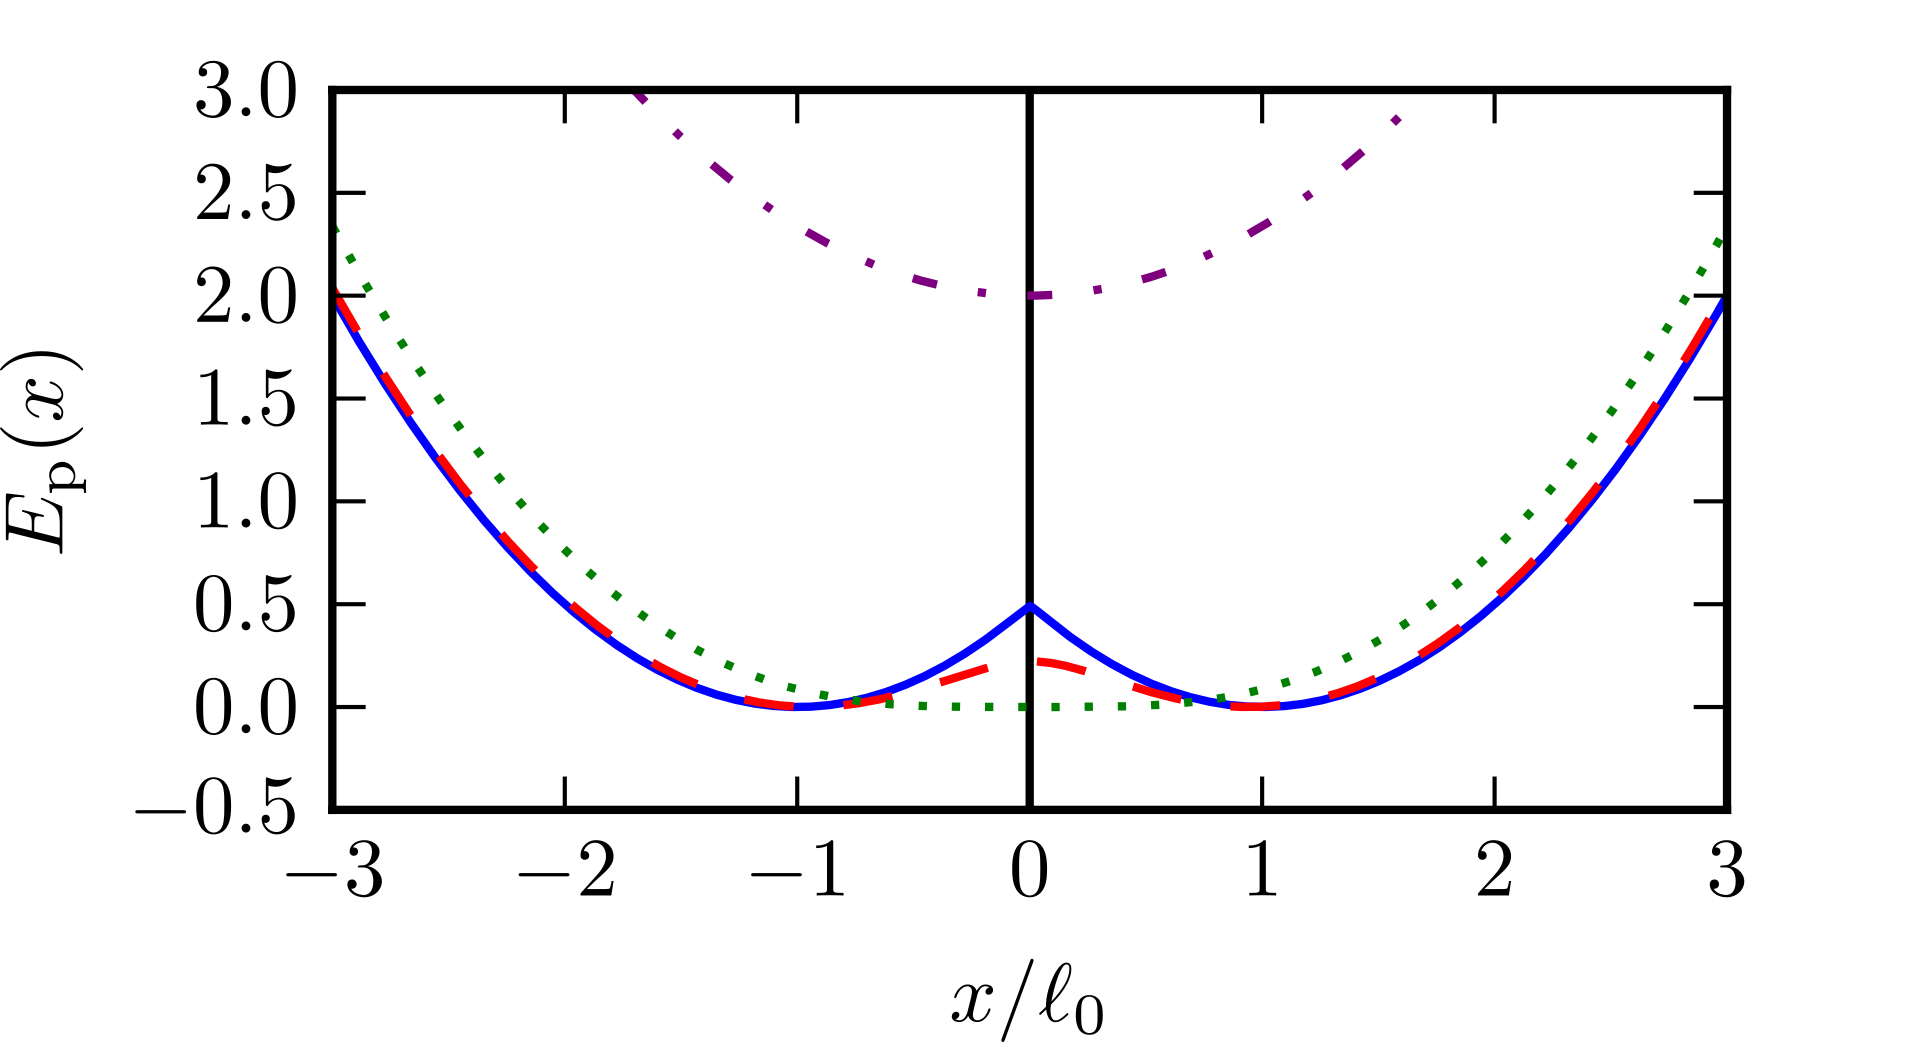
\includegraphics[width=\linewidth]{landeau_ep-plain}
		\end{center}
	\end{minipage}
	\hfill
	\begin{minipage}{0.45\linewidth}
		\begin{center}
			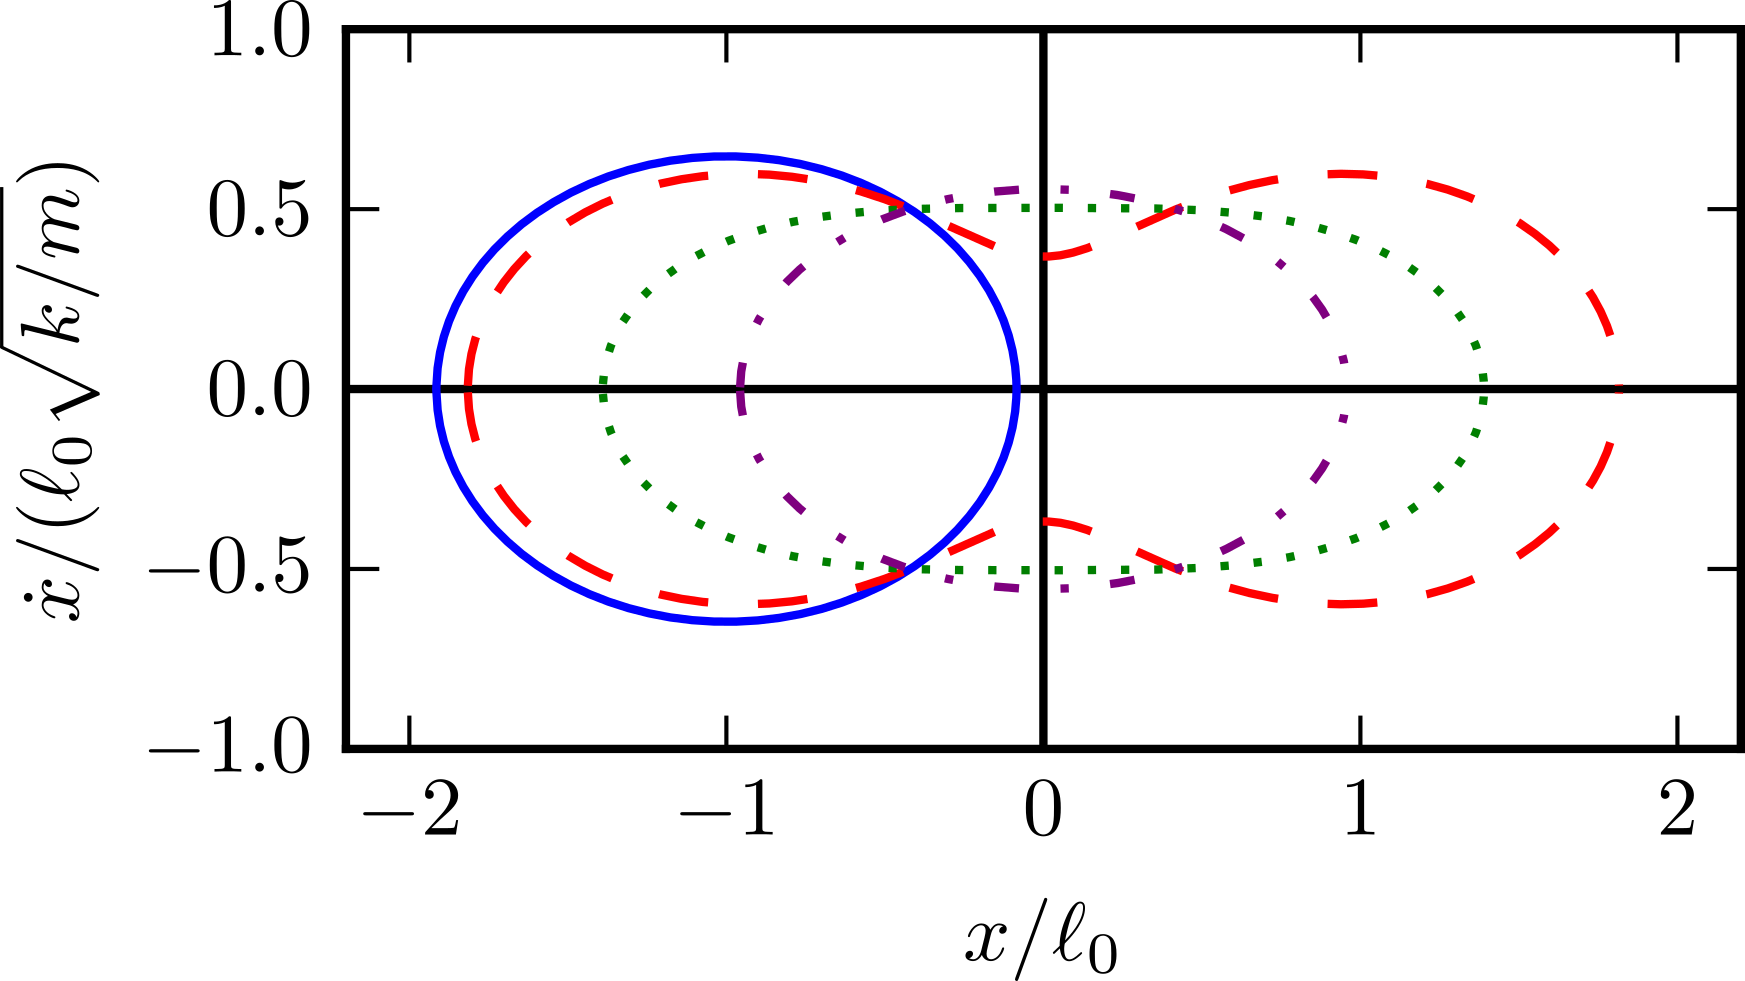
\includegraphics[width=\linewidth]{landeau_xp-plain}
		\end{center}
	\end{minipage}
}

\end{document}
